\documentclass{article}
\usepackage[utf8]{inputenc}
\usepackage{fancyvrb}
\usepackage[pdfborder={0 0 0}]{hyperref}
\usepackage{url}
\usepackage{upquote}
\usepackage{graphicx}
\usepackage{float}
\usepackage{natbib}
%% \VignetteIndexEntry{sdcTab Vignette}

\newcommand{\sdcTab}{\texttt{sdcTab}}
%% path, filename, caption, label

\newcommand{\listing}[4]{        %
  \begin{figure}[H]              %
    \centering                   %
    \VerbatimInput[numbers=left, %
      frame=single,              %
      label=#2]{#1}              %
    \caption{#3}                 %
    \label{#4}                   %
  \end{figure}                   %
}
\author{Bernhard Meindl \url{<bernhard.meindl@statistik.gv.at>}}

\newcommand{\sdcTable}{{\tt sdcTable}}

\title{\sdcTable~Vignette}
\usepackage{Sweave}
\begin{document}
\maketitle
\begin{abstract}
  The purpose of the \sdcTable~vignette is to show how to get up and
  running with \sdcTable; for details, including a complete list of
  options, consult the help pages or the manual for the following 
  main functions of the package:
  \begin{itemize}
  \item {\tt makeProblem} using e.g: help('makeProblem')
  \item {\tt primarySuppression} using e.g: help('primarySuppression')
  \item {\tt protectTable} using e.g: help('protectTable')
  \item {\tt setInfo} using e.g: help('setInfo')
  \item {\tt getInfo} using e.g: help('getInfo')
  \end{itemize}
\end{abstract}
\tableofcontents

\newpage

\section{Introduction to \sdcTable}
{\tt R}-package \sdcTable~is free and open source software that provides 
methods to generate instances of multidimensional, hierarchical table structures,
identify primary sensitive table cells within such objects and finally protect
primary sensitive table cells by solving the secondary cell suppression problem
with currently 3 implemented algorithms. 

\section{How to protect data - An overview}

\begin{figure}[H]
 \centering
 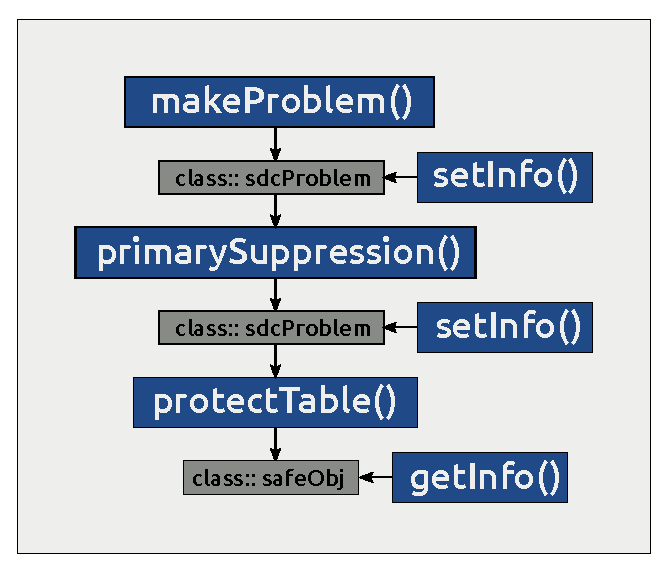
\includegraphics[width=8cm]{overview}
 \caption{\sdcTable~- overview of exported functions}
 \label{fig:overview}
\end{figure}

The main functions that are exported to users are shown in Figure (\ref{fig:overview}). \\

Function {\tt makeProblem()} is used to create objects of class {\tt sdcProblem}.
Instances class {\tt sdcProblem} hold the entire information that is required to 
perform primary or secondary cell suppression such as assumed to be known upper
and lower cell bounds or upper-, lower- or sliding protection levels that are 
required to fulfill when solving the secondary cell suppression problem. All these
information can be modified using function {\tt setInfo()}. \\

{\tt primarySuppression()} is applied to objects of class {\tt sdcProblem}. By 
setting function parameters users can choose and apply a pre-defined primary
suppression rule. Using {\tt setInfo()} one can easily implement a custom primary 
suppression rule, too. \\

Function {\tt protectTable()} is used to protect primary sensitive table cells in 
objects of class {\tt sdcProblem}. A successful run of  function {\tt protectTable()} 
results in an object of class {\tt safeObj}.  Using {\tt getInfo()} one can 
extract information from objects  of such class, most importantly of course 
a data set containing all table cells along with the suppression pattern. \\

More detailed information on all the possibilities is available in the help-files,
additional information is given in the corresponding sections of this vignette 
that deal with specific functions. The first step however to get started is to  
load the package, which can easily be done as  shown below:
\begin{Schunk}
\begin{Sinput}
> library(sdcTab)
\end{Sinput}
\begin{Soutput}
Using the GLPK callable library version 4.42
Package sdcTab 0.9.5 has been loaded!
\end{Soutput}
\end{Schunk}

\section{A simple example}
We now walk through the steps that are required to protect tabular data using 
\sdcTable. In the first example we are going to protect table cells given a 
three-dimensional tabular structure with some sub-totals. \\

We will start by discussing input data sets in sections (\ref{ex1:microDat}) 
and (\ref{ex1:aggDat}). Then we continue by discussing how to define and 
describe dimensional variables in (\ref{ex1:hier}) which is a crucial 
step in the entire procedure. Once the hierarchies are defined it is necessary
to create suitable objects (\ref{ex1:makeProb}) that can be used to identify 
and suppress primary sensitive cells. This is shown in section in section 
(\ref{ex1:primSupp}). Finally we discuss how to protect cells that are primary 
sensitive in section (\ref{ex1:secondSupp}). \\

Throughout it is also shown how to set and extract information from the objects we 
are working with using functions {\tt getInfo()} and {\tt setInfo()}.

\subsection{Starting from microdata}\label{ex1:microDat}
In this example we suppose we have collected data from 1000 
individuals. A subset of the available data is shown below:
\begin{Schunk}
\begin{Sinput}
> print(head(microData), row.names=FALSE)
\end{Sinput}
\begin{Soutput}
 V1 V2 V3 numVal2 numVal1
  A  w  d   49.93   71.72
  C  m  f   48.44   55.96
 Ba  m  a   43.20   64.69
 Bc  w  d   31.38   30.72
 Bc  w  a   49.46   54.93
 Ba  m  d   42.02   22.23
\end{Soutput}
\end{Schunk}
We note that the information we have obtained for any individual corresponds to 
exactly one row in the input data.frame. That is supposed to available in 
{\tt R}. \\

The micro data consist of 5 variables. The first 3 variables
('V1', 'V2' and 'V3') are categorical variables that will later define the table 
that needs to be protected. Variables 'numVal1' and 'numVal2' correspond to 
arbitrary variables containing some kind of information measured for each 
individual. \\

To create the tabular structure that is required to protect any table cells
within the table it is of course of interest to have a look at possible values or
characteristics of the categorical variables that define the table.


\begin{itemize}
	\item Variable 'V1': this variable has a total of 6 
	codes without subtotals which are listed below:
\begin{Schunk}
\begin{Soutput}
[1] "A"  "Ba" "Bb" "Bc" "C"  "D" 
\end{Soutput}
\end{Schunk}
	\item Variable 'V2': this variable has a total of 2 
	codes without subtotals which are listed below:
\begin{Schunk}
\begin{Soutput}
[1] "m" "w"
\end{Soutput}
\end{Schunk}
	\item Variable 'V3': this variable has a total of 6 
	codes without subtotals which are listed below:
\begin{Schunk}
\begin{Soutput}
[1] "a" "b" "c" "d" "e" "f"
\end{Soutput}
\end{Schunk}
\end{itemize}

The step on how to define level-hierarchies that have to include all possible
(sub)totals is explained in section (\ref{ex1:hier}).

\subsection{Using aggregated data}\label{ex1:aggDat}
Using \sdcTable~it is also possible to start with a 'complete' dataset. This 
means that the input dataset already contains rows with all possible level-combinations
that can occur. This also includes combinations with (sub)totals. In this case
it is required that the input data contain a column holding cell counts. Using the
example data already discussed in (\ref{ex1:microDat}), the complete dataset could
be specified as shown below:

\begin{Schunk}
\begin{Sinput}
> print(tail(completeData))
\end{Sinput}
\begin{Soutput}
     V1  V2 V3 Freq  numVal1  numVal2
163   C Tot  f   24  7523.30  7305.85
164   D Tot  f   31  7723.40  7698.75
165 Tot   m  f  107 24033.37 24325.32
166   B   m  f   55 12797.11 13372.83
167 Tot   w  f   85 25082.25 25459.33
168   B   w  f   50 12600.68 12861.13
\end{Soutput}
\end{Schunk}

Even though we only show a small subset of the data it is immediately clear that 
in object {\tt completeData} (sub)totals are listed. These combinations can be 
calculated from the microdata by summation over several codes in one or more
dimensional variables. As in (\ref{ex1:microDat}) it is of interest which codes
were specified for each dimensional variable. This information is given below:
\begin{itemize}
	\item Variable 'V1': this variable has a total of 8 
	codes including all possible subtotals which are listed below:
\begin{Schunk}
\begin{Soutput}
[1] "Tot" "A"   "B"   "Ba"  "Bb"  "Bc"  "C"   "D"  
\end{Soutput}
\end{Schunk}
	\item Variable 'V2': this variable has a total of 3 
	codes including all possible which are listed below:
\begin{Schunk}
\begin{Soutput}
[1] "Tot" "m"   "w"  
\end{Soutput}
\end{Schunk}
	\item Variable 'V3': this variable has a total of 7 
	codes including all possible which are listed below:
\begin{Schunk}
\begin{Soutput}
[1] "Tot" "a"   "b"   "c"   "d"   "e"   "f"  
\end{Soutput}
\end{Schunk}
\end{itemize}

We also note that in {\tt completeData} a variable 'Freq' is available which 
gives information on the corresponding cell counts. This means that for example
a total of 50 individuals contribute to the table cell where variable
'V1' equals 'B', variable 'V2' is 'w' and variable 'V2' is
equal to 'f'. \\

Whether or not one starts to work with micro data or already with a complete, 
pre-aggregated dataset the next step is always the definition of the hierarchies
defining the tabular structure. 

\subsection{Defining hierarchies}\label{ex1:hier} 
We could see in (\ref{ex1:microDat}) and (\ref{ex1:aggDat}) that the set of codes
available in the input data for varaiables 'V1', 'V2' and 'V3' differ since in
the case where micro data are used as input data, no codes for subtotals are 
included in the micro data while in the case where pre-aggregated data are used 
those subtotals must already be included in the input data set. \\

When defining the complete hierarchies, no (sub)-totals must be excluded 
from the description. This means that for each variable defining one dimension 
of the table the complete structure must of course includes all (sub)totals. \\

In this example the hierarchies we want to define are quite basic. We start by
showing the level-codes for each variable 'V1', 'V2' and 'V3' that are included
in {\tt completeData} but not in {\tt microData}.
\begin{itemize}
	\item (sub)totals of variable 'V1':
\begin{Schunk}
\begin{Soutput}
[1] "Tot" "B"  
\end{Soutput}
\end{Schunk}
	\item (sub)totals of variable 'V2':
\begin{Schunk}
\begin{Soutput}
[1] "Tot"
\end{Soutput}
\end{Schunk}
	\item (sub)totals of variable 'V3':
\begin{Schunk}
\begin{Soutput}
[1] "Tot"
\end{Soutput}
\end{Schunk}
\end{itemize} 

We observe that variable 'V1' has two codes ('Tot' and 
'B') that can be calculated from the codes of 'V1' available
in the micro data set {\tt microData}. For variables 'V2' and 'V3' only one total
value ('Tot') exists which means the summation over all 
characteristics of variables 'V2' and 'V3' is the (only) total value.  \\

To specify the complete structure of a dimensional variable one needs to create
a data frame or a matrix for each of those variables. The structure of any 
object describing a dimensional variable be created as follows:
\begin{enumerate}
	\item the object must consist of exactly 2 columns, both being character
	vectors
	\item the first column specifies levels
	\item the second column specifies level-codes
	\item the only allowed character in the first column is '@'
	\item the length of the strings of the first column defines the (numeric) level
	of the corresponding code
	\item a top-down approach has to be taken
	\item the object must contain a row for each possible level-code 
\end{enumerate}
While this may sound difficult, it is in fact quite easy to create such objects
within {\tt R}. We will now explain how to create the required objects for the 
dimensional variables 'V1', 'V2' and 'V3' used in the example. 

\subsubsection*{defining level-structure for variable 'V1'}
The hierarchy we want to describe is as follows. The overall code 'Tot'
is calculated from the codes ('A', 'B', 'C' and 'D'). Additionally, code 'B' (which
is the second (sub)total-code for variable 'V1' as shown in section  (\ref{ex1:aggDat}))
can be calculated from the level-codes 'Ba', 'Bb' and 'Bc'. \\

Following rule 1, we have to create a data frame or matrix  consisting of two 
columns, the first specifying levels, the second column the corresponding level 
codes. Since we have to follow a top-down approach, the first level code must 
always correspond to the grand total which is always considered as the code with 
a level equaling 1. Thus, we create the matrix with a single row defining the 
overall total as follows:
\begin{Schunk}
\begin{Sinput}
> dimV1 <- matrix(nrow = 0, ncol = 2)
> dimV1 <- rbind(dimV1, c("@", "Tot"))
> print(dimV1)
\end{Sinput}
\begin{Soutput}
     [,1] [,2] 
[1,] "@"  "Tot"
\end{Soutput}
\end{Schunk}

The level code for the overall total is '@' because according to rule 4 it is the
only allowed character in the first column and it consists of exactly 1 character.
Also, since the overall total is defined as level 1, the number of characters of
the string '@' and the level of the overall total code 'Tot' matches. \\

The next step is to add additional codes. As mentioned before, codes 'A', 'B', 
'C' and 'D' contribute the the overall total. Therefore we know that these codes
are considered as level 2 codes and must be (according to the top-down approach)
listed below the overall total code. Adding these codes to object {\tt dimV1} 
{\tt dimV1} is shown below:
\begin{Schunk}
\begin{Sinput}
> mat <- matrix(nrow = 4, ncol = 2)
> mat[, 1] <- rep("@@", 4)
> mat[, 2] <- LETTERS[1:4]
> dimV1 <- rbind(dimV1, mat)
> print(dimV1)
\end{Sinput}
\begin{Soutput}
     [,1] [,2] 
[1,] "@"  "Tot"
[2,] "@@" "A"  
[3,] "@@" "B"  
[4,] "@@" "C"  
[5,] "@@" "D"  
\end{Soutput}
\end{Schunk}

We know that code 'B' is a subtotal that can be calculated from codes
'Ba', 'Bb' and 'Bc'. Since 'B' is a code of level 2, the codes contributing to
it must be of a lower level, in this case of level 3. We show below how to add
the codes to object {\tt dimV1}:

\begin{Schunk}
\begin{Sinput}
> mat <- matrix(nrow = 3, ncol = 2)
> mat[, 1] <- rep("@@@", 3)
> mat[, 2] <- c("Ba", "Bb", "Bc")
> dimV1 <- rbind(dimV1, mat)
> print(dimV1)
\end{Sinput}
\begin{Soutput}
     [,1]  [,2] 
[1,] "@"   "Tot"
[2,] "@@"  "A"  
[3,] "@@"  "B"  
[4,] "@@"  "C"  
[5,] "@@"  "D"  
[6,] "@@@" "Ba" 
[7,] "@@@" "Bb" 
[8,] "@@@" "Bc" 
\end{Soutput}
\end{Schunk}
Now object {\tt dimV1} contains all possible codes along with their levels. However,
it not valid because the top-down approach is violated. This means that codes that
contribute to a (sub)total must be listed directly below it. If we would not change
the order of object {\tt dimV1}, \sdcTable~would assume that code 'D' can be calculated
by summation over codes 'Ba', 'Bb' and 'Bc'. For this reason it is necessary to
move this 'block' up so that it is directly below code 'B'. The required code 
and the resulting correct object describing the structure of variable 'V1' is 
printed below:
\begin{Schunk}
\begin{Sinput}
> dimV1 <- dimV1[c(1:3, 6:8, 4:5), ]
> print(dimV1, row.names = FALSE)
\end{Sinput}
\begin{Soutput}
     [,1]  [,2] 
[1,] "@"   "Tot"
[2,] "@@"  "A"  
[3,] "@@"  "B"  
[4,] "@@@" "Ba" 
[5,] "@@@" "Bb" 
[6,] "@@@" "Bc" 
[7,] "@@"  "C"  
[8,] "@@"  "D"  
\end{Soutput}
\end{Schunk}

Using this information, \sdcTable~internally calculates all kinds of information
on dimensional variables. So for example it is able to deal with codes that can
be (temporarily) removed from the structure because it can be considered as a
'duplicate'. This is however not the case for this basic dimensional variable
that has a total of 8 codes of which 6 are required to calculate information
for the 2 (sub)totals.

\subsubsection*{defining level-structure for variable 'V2'}
The creation of a suitable object that describes the hierarchical structure
of variable 'V2' is easy. We are only dealing with one overall Total ('Tot')
that is the sum of all codes listed in (\ref{ex1:microDat}) for this variable.\\

The code how to specify an object that describes the structure of dimensional 
variable 'V2' is given below:
\begin{Schunk}
\begin{Sinput}
> dimV2 <- matrix(nrow = 3, ncol = 2)
> dimV2[, 1] <- c("@", "@@", "@@")
> dimV2[, 2] <- c("Tot", "m", "w")
> print(dimV2, row.names = FALSE)
\end{Sinput}
\begin{Soutput}
     [,1] [,2] 
[1,] "@"  "Tot"
[2,] "@@" "m"  
[3,] "@@" "w"  
\end{Soutput}
\end{Schunk}

We see that the overall total ('Tot') is again listed in the first row as level 1
('@' has one character) while all contributing codes ('m' and 'w') are listed 
below the total and are of level 2 ('@@' has two characters).

\subsubsection*{defining level-structure for variable 'V3'}
The creation of a suitable object that describes the hierarchical structure
of variable 'V3' is easy. We are only dealing with one overall Total ('Tot')
that is the sum of all codes listed in (\ref{ex1:microDat}) for variable 'V3'.\\

The required code to generate an object specifying the hierarchical structure of 
variable 'V3' is given below:

\begin{Schunk}
\begin{Sinput}
> dimV3 <- matrix(nrow = 7, ncol = 2)
> dimV3[, 1] <- c("@", rep("@@", 6))
> dimV3[, 2] <- c("Tot", letters[1:6])
> print(dimV3, row.names = FALSE)
\end{Sinput}
\begin{Soutput}
     [,1] [,2] 
[1,] "@"  "Tot"
[2,] "@@" "a"  
[3,] "@@" "b"  
[4,] "@@" "c"  
[5,] "@@" "d"  
[6,] "@@" "e"  
[7,] "@@" "f"  
\end{Soutput}
\end{Schunk}

It is required to create an object defining the complete structure and 
hierarchies for each dimensional variable. One this step has been done, the 
multidimensional tabular structure that is required to apply any statistical 
disclosure methods can be created using {\tt makeProblem()}.

\subsection{Creating objects of class {\tt sdcProblem} for further processing}
\label{ex1:makeProb}

We now show how to create objects of class {\tt sdcProblem} which can further
be used to identify, suppress and protect sensitive table cells. \\

It was discussed in (\ref{ex1:microDat}) and (\ref{ex1:aggDat}) how 
micro data and pre-aggregated data can be used as data-input objects. We will now
explain how to create instances of class {\tt sdcProblem} from both  {\tt microData} 
and {\tt completeData} and describe the required and optional parameters of 
function {\tt makeProblem}.\\

We start building an suitable object of class {\tt sdcProblem} starting with 
the micro data set {\tt microData} discussed in section (\ref{ex1:microDat}).
\begin{Schunk}
\begin{Sinput}
> dimInfo <- list(V1 = dimV1, V2 = dimV2, V3 = dimV3)
> prob.microDat <- makeProblem(data = microData, dimList = dimList, 
+     dimVarInd = 1:3, freqVarInd = NULL, numVarInd = 4:5, weightInd = NULL, 
+     sampWeightInd = NULL, isMicroData = TRUE)
\end{Sinput}
\end{Schunk}

First we have to combine the objects describing the hierarchical variables 'V1',
'V2' and 'V3' into a list called {\tt dimList}. Each list element is one of the
objects created in section (\ref{ex1:hier}). The names of the list-elements must
correspond to the variable name that the corresponding list-element refers to. In
this case, the first list-element - 'dimV1' - should describe variable 'V1' in 
the input data set {\tt microData} when calling {\tt makeProblem()} while the
second list element - 'dimV2' - defines the hierarchy of variable 'V2' and 'dimV3' 
- the third list element - describes the structure of variable 'V3'.\\

The remaining parameters are quite self-explanatory and shorty described:
\begin{itemize}
	\item {\bf data}: the data set that should be used, in this case {\tt microData}
	\item {\bf dimList}: a named list containing information on the structure 
	of dimensional variables as described just above
	\item {\bf dimVarInd}: the column indices of dimensional described in {\tt dimList}.	
	\item {\bf freqVarInd}: if not {\tt NULL} an index specifying the column
	that contains information on cell counts 
	\item {\bf numVarInd}: if not {\tt NULL} an index specifying the columns
	holding other numerical variables  
	\item {\bf weightInd}: if not {\tt NULL} an index specifying the column that
	contains info on weights that should be used in the secondary cell suppression
	problem instead of cell counts
	\item {\bf sampWeightInd}: if not {\tt NULL} an index specifying the column
	holding sampling weights for each person | group  
	\item {\bf isMicroData}: {\tt TRUE} if input are micro data and {\tt FALSE} otherwise.
\end{itemize}

Building an object of class {\tt sdcProblem} using the complete, pre-aggregated 
data {\tt completeData} as discussed in section (\ref{ex1:aggDat}) is very 
similar as it is shown below:

\begin{Schunk}
\begin{Sinput}
> dimInfo <- list(V1 = dimV1, V2 = dimV2, V3 = dimV3)
> prob.completeDat <- makeProblem(data = completeData, dimList = dimList, 
+     dimVarInd = 1:3, freqVarInd = 4, numVarInd = 5:6, weightInd = NULL, 
+     sampWeightInd = NULL, isMicroData = FALSE)
\end{Sinput}
\end{Schunk}
The only difference is that in this case we define parameter 'freqVarInd' that
specifies a column within the input data set {\tt completeData} containing
information on cell counts. Also the indices of argument 'numVarInd' are different
that in the first example and argument 'isMicroData' is now of course {\tt FALSE}
since we are dealing with pre-aggregated data.\\

In any case, both procedure return an object of class {\tt sdcProblem} as can
easily be checked:
\begin{Schunk}
\begin{Sinput}
> all(c(class(prob.microDat), class(prob.completeDat)) == "sdcProblem")
\end{Sinput}
\begin{Soutput}
[1] TRUE
\end{Soutput}
\end{Schunk}

We now can check if the cell counts of both objects are equal. Function 
{\tt getInfo()} can be used to extract information from objects of class 
{\tt sdcProblem}. Specifying argument 'type' as 'freq', {\tt getInfo()} returns 
cell counts which of course are equal independent if micro-data or pre-aggregated
data have been used as input to create the complete tabular structure.
\begin{Schunk}
\begin{Sinput}
> counts1 <- getInfo(prob.completeDat, type = "freq")
> counts2 <- getInfo(prob.microDat, type = "freq")
> all(counts1 == counts2)
\end{Sinput}
\begin{Soutput}
[1] TRUE
\end{Soutput}
\end{Schunk}

Once the problem has been set up and an instance of class {\tt sdcProblem} is 
available, it is possible to identify and suppress sensitive table cells as
we demonstrate in the next section using object {\tt prob.completeDat}. 

\subsection{Primary suppression}\label{ex1:primSupp}
Identifying and suppression primary sensitive cells is usually done by applying
function {\tt primarySuppression()}.  \\

Having a look at the cell counts in table {\tt prob.completeDat} shows that a 
total of
\begin{Schunk}
\begin{Sinput}
> length(which(counts1 <= 10))
\end{Sinput}
\begin{Soutput}
[1] 15
\end{Soutput}
\end{Schunk}
cells have less than 10 individuals contributing to it. We think that these
cells should be considered as primary sensitive and we want to have them protected.
When creating an object of class {\tt sdcProblem} all cells are assigned an
anonymization state. The possible codes are listed below:
\begin{itemize}
	\item {\bf 'u'}: cell is primary suppressed and needs to be protected
	\item {\bf 'x'}: cell has been secondary suppressed
	\item {\bf 's'}: cell can be published
	\item {\bf 'z'}: cell must not be suppressed 
\end{itemize}

The goal is now to change the anonymization status of all cells having less than
10 individuals contributing to it from the default value of 's' to 'u'. The
easiest way is to use function {\tt primarySuppression()} directly:

\begin{Schunk}
\begin{Sinput}
> prob.completeDat <- primarySuppression(prob.completeDat, type = "freq", 
+     maxN = 10)
\end{Sinput}
\end{Schunk}
Argument 'type' specifies the primary suppression rule we want to apply. In this
case we want to use the frequency threshold rule that allows to suppress all
table cells having cell counts less or equal than the threshold specified using 
argument 'maxN'. {\tt primarySuppression()} also allows to apply the nk-dominance 
rule or the p-percent rule directly, in case micro data have been used as input 
data. For all possible parameters and their explanation the interested reader 
may  consult the manual or the help-page of {\tt primarySuppression()}. \\

After performing the suppression, we can have a look at the distribution
of the anonymization states:

\begin{Schunk}
\begin{Sinput}
> print(table(getInfo(prob.completeDat, type = "sdcStatus")))
\end{Sinput}
\begin{Soutput}
  s   u 
153  15 
\end{Soutput}
\end{Schunk}


One can see that the 15 cells having counts less or equal than
10 have been identified and marked as primary suppressed. However, we should note
that it is very easy to implement custom suppression rules by manually changing
the anonymization state of cells using functions {\tt setInfo()} or 
{\tt changeCellStatus()}. Information on how to use these functions is of course
provided in the manual and the corresponding help-pages. \\ 

To protect these cells by solving the secondary cell suppression problem one can 
go on to use function {\tt protectTable()} as explained in the next section.

\subsection{Secondary cell suppression using \sdcTable}\label{ex1:secondSupp}
\sdcTable~provides the algorithms to protect primary sensitive table cells within
objects of class {\tt sdcProblem}. The algorithms that may be selected are:
\begin{itemize}
	\item {\bf OPT}: protect the complete hierarchical, multidimensional table 
	at once. This algorithm is however only suitable for small problem instances.
	\item {\bf HITAS}: solving the secondary cell suppression problem by applying
	a cut and branch algorithm to subtables that are protected in specific order
	\item {\bf HYPERCUBE}: solving the problem using a heuristic that is based on
	finding geometric hypercubes that are required to protect primary sensitve 
	table cells
\end{itemize}

We show how to protect the data using the three possible variants and its default
parameters. For an extensive discussion on the possible parameters have a look
at the manual or help page for function {\tt protectTable()}.

\begin{Sinput}
> resHITAS <- protectTable(prob.completeDat, method="HITAS")
> resOPT <- protectTable(prob.completeDat, method="OPT")
> resHYPER <- protectTable(prob.completeDat, method="HYPERCUBE")
\end{Sinput}

Having a look at the Output objects we can observe that the number of secondary
suppressions required to protect the 15 primary sensitive cells
(by default against exact re-calculation given sliding protection levels of 1 for
each primary sensitive cell) differs. \\

Using the 'OPT'-algorithm, a total of 23
cells have been marked as secondary suppressions. When using 'HITAS'-algorithm, it
was required to additionally suppress  25
cells. A total of  29 cells was 
selected and marked as secondary suppressions when the 'HYPERCUBE' algorithm was
used. \\

One now easily get information from the resulting output objects that are instances
of class {\tt safeObj} by using function {\tt getInfo()} or applying the 
{\tt summary}-method. For the former we show how to extract the final data set 
which can be achieved as follows:
\begin{Schunk}
\begin{Sinput}
> finalData <- getInfo(resOPT, type = "finalData")
> print(head(finalData))
\end{Sinput}
\begin{Soutput}
  V1 V2 V3 Freq numVal1 numVal2 sdcStatus
1  A  m  a   12 3919.84 4090.31         s
2 Ba  m  a   18 4707.53 5101.81         s
3 Bb  m  a   18 4199.31 4186.62         x
4 Bc  m  a   10 3890.27 4084.40         u
5  C  m  a   11 3341.39 2988.84         s
6  D  m  a   13 3975.03 3873.34         s
\end{Soutput}
\end{Schunk}
As we can see above the final result data set contains all columns specified in
the input data set along with another column 'sdcStatus' that specifies the
anonymization state for each table cell. \\

For the latter we show how to apply the summary method. This can be done by
applying the following code:
\begin{Schunk}
\begin{Sinput}
> summary(resOPT)
\end{Sinput}
\begin{Soutput}
######################################################
### Summary of the result object of class 'safeObj' ###
######################################################
--> The input data have been protected using algorithm OPT.
--> The algorithm ran for 45 seconds.
--> To protect 15 primary sensitive cells, 23 cells need to be additionally suppressed.
--> A total of 130 cells may be published.

###################################
### Structure of protected Data ###
###################################
'data.frame':	168 obs. of  7 variables:
 $ V1       : Factor w/ 8 levels "A","B","Ba","Bb",..: 1 3 4 5 6 7 1 3 4 5 ...
 $ V2       : Factor w/ 3 levels "m","Tot","w": 1 1 1 1 1 1 3 3 3 3 ...
 $ V3       : Factor w/ 7 levels "a","b","c","d",..: 1 1 1 1 1 1 1 1 1 1 ...
 $ Freq     : num  12 18 18 10 11 13 19 12 12 18 ...
 $ numVal1  : num  3920 4708 4199 3890 3341 ...
 $ numVal2  : num  4090 5102 4187 4084 2989 ...
 $ sdcStatus: chr  "s" "s" "x" "u" ...
NULL
\end{Soutput}
\end{Schunk}
We see that the summary provides all kind of useful information such as the
algorithm that has been used to protect primary sensitive cells, the time it 
has been taken to solve the problem, the number of primary sensitive and 
secondary suppressed cells as well as the number of cells that may be published.
Also, a excerpt of the final data set is shown. \\

I would also like to mention that an iterative algorithm is available in function
{\tt protectLinkedTables()} that allows to protect two tables that have common 
table cells. The function takes two objects of class {\tt sdcProblem} as input 
and a list defining the common cells in both tables. Details on how to construct 
this a list-element are given in the manual and help-page
of {\tt protectLinkedTables()}. 

%%%%%%%%%%%%%%%%%%%%%%%%%%%%%%%%
%%% Protecting Linked Tables %%%
%%%%%%%%%%%%%%%%%%%%%%%%%%%%%%%%
%\section{Protecting linked tables}
%\subsection{Starting from micro data}
%\subsection{Defining required hierarchies}
%\subsection{Identifying and suppressing sensitive cells}
%\subsection{Performing secondary cell suppression for the linked tables}

\section{Remarks}
A lot of work has gone into the rewrite of \sdcTable~using S4-classes and methods
in order to robustify the code and in order to make it easier in future to add
new algorithms such as rounding- or cell-perturbation methods and features.\\

I would really like to hear any kind of feedback and wil be more than happy to 
work in patches you submit or ideas any one might have which would make it easier to 
work \sdcTable. Also, the next step in the evolution of the package will be performance
optimization, evaluation for possibilities of parallel computing and so on. I would really
like to hear any kind of feedback on package users on these kind of things. Thus, 
for any remarks, plesae do not hesitate to contact me using my e-mail adress
\url{bernhard.meindl@statistik.gv.at}.

%\bibliographystyle{plainnat}
\bibliography{sdcTab}
\end{document}
